%! alt A regular hexagon with a good point X inside it. Rays from X to the six corners cut the hexagon into six triangles, one on each side. The triangle on side 5, at the lower left, is shaded and is cut by five more rays into six pieces of equal area. Perpendiculars from X to sides 1, 2 and 3, where side 1 is the right-hand side and the sides are numbered anticlockwise, have lengths d1, d2 and d3, here 12, 14 and 12 twentieths of the distance between opposite sides, and d1 - d2 + d3 is half that distance.
%! after_paragraph 2
%! scale 1/3
%! let r = 20/sqrt(3)
% The shared preamble of every Cevian figure. pipeline/figures turns these colours into theme-aware paint,
% and refuses any other colour, so draw only with them:
%   figink (lines and labels), figaux (construction lines), figaccent (the object the argument turns on),
%   figtint and figaccenttint (light fills).
\documentclass[border=1.5pt]{standalone}
\usepackage{tkz-euclide}
\definecolor{figink}{RGB}{0,0,0}
\definecolor{figaux}{RGB}{85,85,85}
\definecolor{figaccent}{RGB}{192,57,43}
\definecolor{figtint}{RGB}{221,221,221}
\definecolor{figaccenttint}{RGB}{245,213,208}
% tkz-euclide's defaults draw circles, compasses and marks in 50% grey and fill points with a tint.
\makeatletter
\def\tkz@otherlinecolor{figink}
\def\tkz@euc@circlecolor{figink}
\def\tkz@euc@compasscolor{figink}
\def\tkz@euc@mkcolor{figink}
\def\tkz@mk@fill{figink}
\def\tkz@euc@pointfillcolor{figink}
\makeatother
\tkzSetUpLine[color=figink,line width=.7pt]
\tkzSetUpArc[color=figink,line width=.7pt]
\tkzSetUpCompass[color=figink,line width=.5pt]
\tkzSetUpPoint[color=figink,fill=figink,size=3.1pt]
\tikzset{
  every picture/.style={line cap=round,line join=round,color=figink},
  circle style/.append style={color=figink,line width=.7pt},
  aux/.style={color=figaux,line width=.45pt,dash pattern=on 2.6pt off 2pt},
  key/.style={color=figaccent,line width=1pt},
  mk/.style={color=figink,line width=.5pt},
  lbl/.style={color=figink,inner sep=2.2pt},
  len/.style={color=figink,inner sep=1.5pt,font=\small},
}

\begin{document}
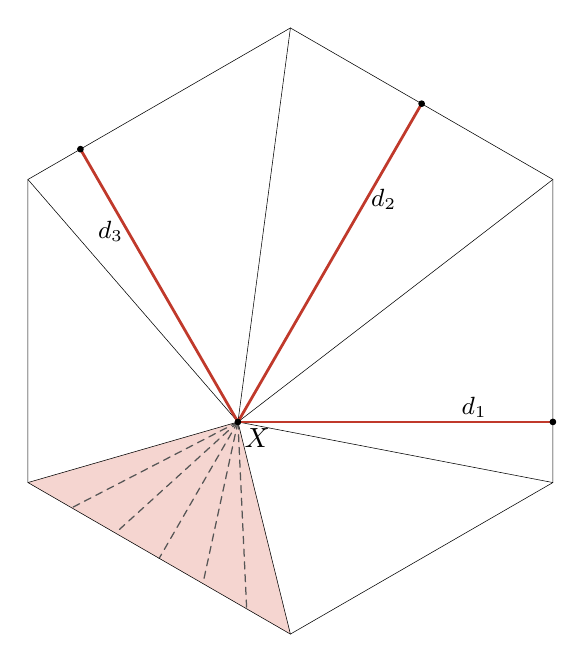
\begin{tikzpicture}
\tkzDefPoint(0.0,0.0){O} %! O = (0, 0)
\tkzDefPoint(3.3333333,-1.9245009){V1} %! V1 = polar(O, r, -30)
\tkzDefPoint(3.3333333,1.9245009){V2} %! V2 = polar(O, r, 30)
\tkzDefPoint(0.0,3.8490018){V3} %! V3 = (0, r)
\tkzDefPoint(-3.3333333,1.9245009){V4} %! V4 = polar(O, r, 150)
\tkzDefPoint(-3.3333333,-1.9245009){V5} %! V5 = polar(O, r, 210)
\tkzDefPoint(0.0,-3.8490018){V6} %! V6 = (0, -r)
\tkzDefPoint(-0.66666667,-1.1547005){X} %! X = (-2, -2*sqrt(3))
\tkzDefPoint(3.3333333,-1.1547005){F1} %! F1 = foot(X, V1, V2)
\tkzDefPoint(1.6666667,2.8867513){F2} %! F2 = foot(X, V2, V3)
\tkzDefPoint(-2.6666667,2.3094011){F3} %! F3 = foot(X, V3, V4)
\tkzDefPoint(-2.7777778,-2.2452510){D1} %! D1 = lerp(V5, V6, 1/6)
\tkzDefPoint(-2.2222222,-2.5660012){D2} %! D2 = lerp(V5, V6, 2/6)
\tkzDefPoint(-1.6666667,-2.8867513){D3} %! D3 = lerp(V5, V6, 3/6)
\tkzDefPoint(-1.1111111,-3.2075015){D4} %! D4 = lerp(V5, V6, 4/6)
\tkzDefPoint(-0.55555556,-3.5282516){D5} %! D5 = lerp(V5, V6, 5/6)
%! fact dist(X, F1) - dist(X, F2) + dist(X, F3) == 10
%! fact perp(X, F1, V1, V2)
%! fact perp(X, F2, V2, V3)
%! fact perp(X, F3, V3, V4)
%! fact on_segment(F1, V1, V2)
%! fact on_segment(F2, V2, V3)
%! fact on_segment(F3, V3, V4)
%! fact dist(V1, V4) == 2 * r
%! example dist(X, F1) == 12
%! example dist(X, F2) == 14
%! example dist(X, F3) == 12
%! example area(X, V1, V2) == 12 * area(V1, V2, V3, V4, V5, V6) / 60
%! example area(X, V2, V3) == 14 * area(V1, V2, V3, V4, V5, V6) / 60
%! example area(X, V3, V4) == 12 * area(V1, V2, V3, V4, V5, V6) / 60
%! example area(X, V5, V6) == 6 * area(V1, V2, V3, V4, V5, V6) / 60
%! example equal(area(X, V5, D1), area(X, D3, D4))
%! example equal(area(X, D5, V6), area(X, D2, D3))
\tkzFillPolygon[color=figaccenttint](X,V5,V6)
\tkzDrawSegments[aux](X,D1 X,D2 X,D3 X,D4 X,D5)
\tkzDrawSegments(X,V1 X,V2 X,V3 X,V4 X,V5 X,V6)
\tkzDrawPolygon(V1,V2,V3,V4,V5,V6)
\tkzDrawSegments[key](X,F1 X,F2 X,F3)
\tkzDrawPoints(X,F1,F2,F3)
\tkzLabelPoint[below right,lbl](X){$X$}
\tkzLabelSegment[above,pos=.75,len](X,F1){$d_1$}
\tkzLabelSegment[right,pos=.7,len](X,F2){$d_2$}
\tkzLabelSegment[left,pos=.7,len](X,F3){$d_3$}
\end{tikzpicture}
\end{document}
